\subsubsection{水的自然与社会属性}

水具有自然属性和社会属性两种不同的属性\cite{ning2004}:自然属性包括水的形态与组成、物理性质与生态功能,以及水参与的地球系统过程等自然特征;而社会属性则包括水的社会功能和社会影响,例如水对个体或集体的认知影响以及水的社会经济功能。

% 开题报告
水在自然界中具有重要的生态功能,不仅参与水文地质循环和生态水文过程,还是大多数陆地生态系统的主要限制因素和物质运移的重要介质,对于生态系统的调节、支持和净化具有至关重要的作用,维持着流域社会生态系统的弹性,使其能够应对外部变化并实现可持续发展\cite{gleeson2020a}。
但是随着人类活动的干预,大河流域的水循环过程受到了严重的破坏,导致其所承担的社会、生态功能已经接近“地球边界”的安全界限\cite{gleeson2020}。
除了自然属性,水还具有重要的社会属性。水不仅是人类生活必需品,而且贯穿了自然、养育、实践和象征等多个方面,具有非常丰富的社会功能和影响\cite{zhangyahui2008}。
水的社会属性可以从“实践理性”和“文化理性”两个方面出发,前者是指在水的生产实践中因控制、竞争、分配、排斥而产生的人水互动;后者是指因水观念、水文化而产生的人水互动\cite{zhangyahui2008}。
除了物质本身的存在,水还具有符号、历史、政治等多种意义,影响着人们的日常生活和流域的政治经济体制\cite{ballestero2019}。

水资源管理是流域特定水文条件、社会文化、经济水平和政治体制的综合产物,通过调整水量的社会分配进而影响生态系统,对于生态系统健康和人类社会福祉具有至关重要的作用。
根据 Stephanie 的总结\cite{scarrow2021},当今人\textendash{}水关系演变的研究可以分为“水的社会性”和“水的技术性”两类。
例如,《大河与大国》\cite{MaDing2021}与《征服自然》\cite{DaWei2019}两项著作分别以美国和德国为例,从“水的社会性”与“社会控制水”两个角度系统梳理了两国主要大河流域的人\textendash{}水关系演变史。前者高度强调“水的社会性”是塑造当代美国社会性质的重要自然因素;后者则指出德国出于征服和控制的考虑,利用技术永远重塑了自然水文景观。
长期以来,流域水资源管理往往通过工程措施短期内提高水的利用规模和效益,而较少考虑系统状态的长期演变,并缺乏反馈机制来处理生态和社会慢变量的积累变迁,限制了维持流域长期可持续的能力\cite{falkenmark2021}。
而可持续水的利用和管理不仅需要考虑其自然特性,还应兼顾其社会功能和经济效益,这需要相关研究耦合水的自然和社会属性,以实现流域可持续发展的目标。

\subsubsection{自然\textendash{}社会二元水循环}

王浩等人提出的“自然\textendash{}社会二元水循环”理论指出,流域水循环受到人类活动影响,呈现出“天然\textendash{}人工”二元特性\cite{wang2006}(图~\ref{ch1:fig:two_water_cycle}~A)。
该理论强调需要以“蒸散发管理”和“耗水管理”为核心来管理自然水循环和人工水循环,提出“以蒸散耗管理为核心、七大总量控制为约束”的水资源管理理念,在水资源评价工作中兼顾了水的自然和社会属性\cite{wang2010}。
该理论的发展也得到了不少学者的补充和完善,例如王浩与贾仰文指出水循环的演变效应也是该理论的研究重点\cite{wang2016},邓铭江等则提出了“自然\textendash{}社会-贸易”三元水循环模式,解释西北干旱区内陆河流域水循环的机理\cite{deng2020}。
该理论的提出强调了水资源管理需要考虑自然和社会属性,应对强烈人类活动干预为水资源评价和管理带来的挑战。

自然\textendash{}社会二元水循环理论以平衡态为基本假设,同时考虑了许多人类活动的影响。在水量估算与建模评价上具有理论优势,主要研究手段是原型观测、物理模型和数学模型。国内学者基于二元水循环的概念模式主要在水资源和水生态方面开展评价管理研究,包括识别循环结构、多尺度多过程分析、演变规律、未来预测与调控等\cite{wang2016}。
例如,刘家宏等人在海河流域应用该理论,构建水平衡方程厘清“自然\textendash{}人工”二元水循环结构,借助数据定量识别了该结构中各部分的数量关系\cite{liu2010}。
王浩\cite{wang2004}、周祖昊\cite{zhou2022b}等人在长达近二十年的时间里,将二元水循环理论从黄河的无定河小流域拓展到整个黄河流域,从初步的二元水循环要素到综合考虑气象、下垫面、人类取用水、水利水保工程、水库调度等诸多要素,不断拓展理论应用的时空尺度。
黄强等人采用小波分析的方法对黄河二元模式的逐年演变规律进行了探索\cite{huang2002};裴源生等人采用该理论改进了水量、水质、水效的联合调控方法\cite{pei2020}。
可见,“自然\textendash{}社会二元水循环”通过考虑人类社会系统对水循环的影响和对水资源的消耗,对指导现代流域水资源管理实践大有裨益。但是,其底层仍基于平衡态的工程思想,在人与水的互馈作用研究上有所不足。

\begin{figure}[!ht]
    \centering
    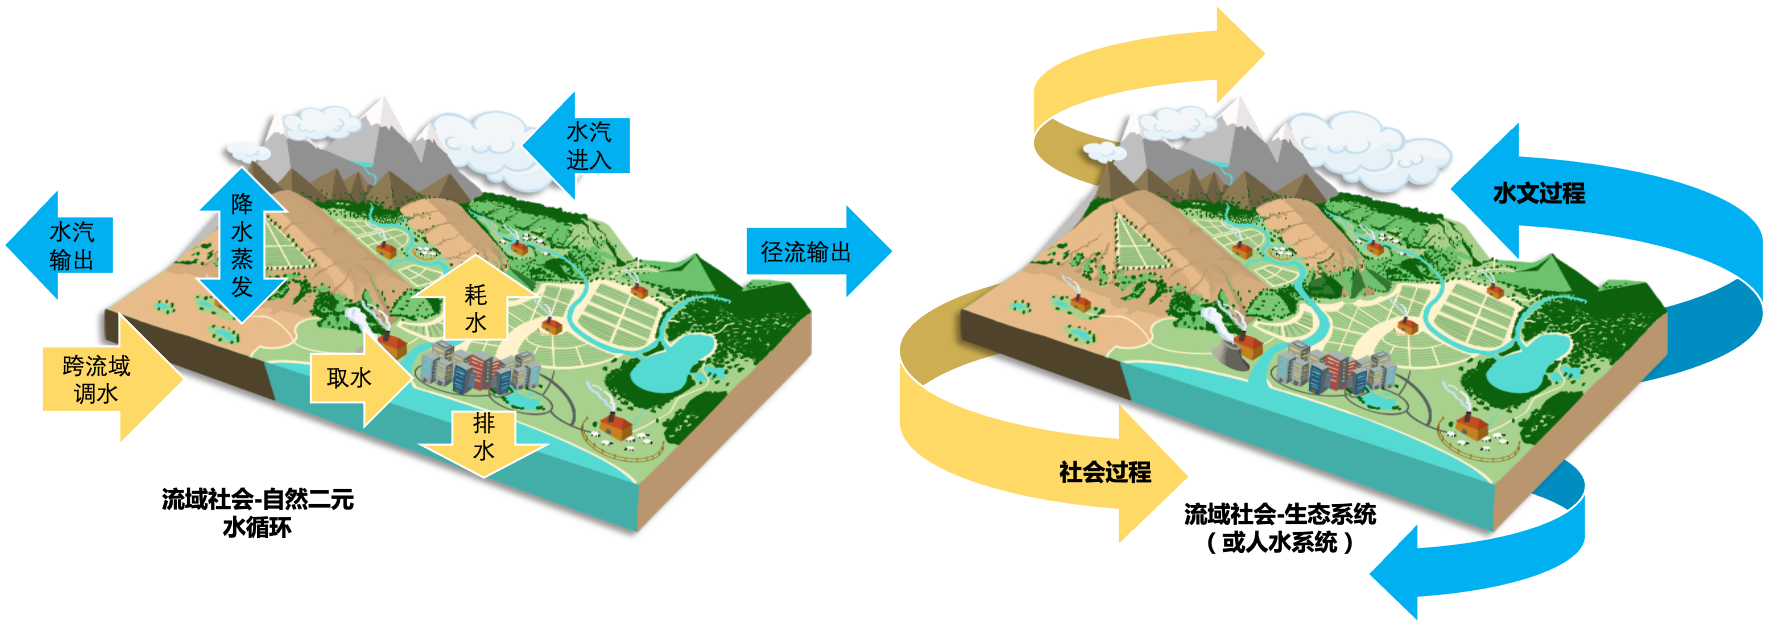
\includegraphics[width=\textwidth]{img/ch1/ch1_two_water_cycle.png}
    \caption[流域人水耦合系统的典型理论示意图]{流域人\textendash{}水系统耦合的典型理论示意图\cite{wang2006,dibaldassarre2015}。蓝色代表自然水循环的典型过程;黄色代表社会水循环的典型过程。}\label{ch1:fig:two_water_cycle}
\end{figure}

\subsubsection{社会水文学}

% 开题报告
社会水文学旨在理解人-水之间协同演化规律和循环互馈机制,多年来在现象检测、机理分析、模型预测等方面都获得了长足发展\cite{sivapalan2012, blair2016, srinivasan2016}。
社会水文学在诞生之初便以流域系统为单元分析人与水的互动反馈过程(图~\ref{ch1:fig:two_water_cycle}~B),其最根本的特征是将社会\textendash{}水文系统视为动态系统,并将人类社会相关变量作为系统内部的驱动力,而非像传统水文学那样假设水文系统是在人类外部干扰下处于平衡态的\cite{sivapalan2012}。
Konar等人将社会水文学的主要研究方向总结为四个:水循环与水资源利用、人与干旱之间的相互作用、人与洪水之间的相互作用、人与政策制度的相互作用\cite{konar2019}。
Yu等人则指出该学科经多年发展后呈现出三个特征:在水循环的不同时空尺度下开展研究、将人类文化的演化特征纳入研究、将基础设施建设对水循环的干扰纳入分析\cite{yu2020}。
在这种超越传统水文学的思想指导下,一些社会\textendash{}水文现象得到揭示,例如增大用水效率却常常无法节约流域水资源的“用水效率悖论”\cite{grafton2018, xiong2021a},以及流域管理策略常在开发和保护之间周期性摆动的“钟摆效应”\cite{kandasamy2014, roobavannan2017, mostert2018}。

社会水文学的发展同时也面临着诸多挑战。
Troy 等人通过文献分析,认为社会水文学研究尚集中在数据收集与整理、数据观察与推测、理论模型建立三个阶段,还缺乏对成熟的参数率定与模型预测,因此其预测能力相对较差,对指导政策制定还相去甚远\cite{troy2015}。
Sanderson 认为这种糟糕的模型表现很大程度上因为社会水文学并没有真正将社会因素纳入考量,因而发出了“社会水文学需要社会科学”的呼吁\cite{sanderson2017}。
然而,社会科学常常没有统一、公认的理论,且人的主观能动性与文化变量均难以被模型捕捉。复杂系统的科学思想能够将复杂的人类行为纳入分析框架,被认为是社会水文学未来重要的前进方向之一\cite{ahlstrom2021}。
综上所述,社会水文学的发展让人们对水问题背后的机制有了更深入的了解。分析与水相连接的社会动态是对传统的水文学的补充。但仍需要进一步在方法学上突破,结合多学科背景和复杂系统思想来分析社会\textendash{}水文系统,以突破上述瓶颈。


\subsubsection{流域社会\textendash{}生态系统}

% Handbook 什么是社会\textendash{}生态系统
社会\textendash{}生态系统(Social-ecological system, SES)的概念最早诞生于20世纪90年代中期,由生态经济学研究公共池塘资源问题的学者通过结合系统科学方法和适应性管理提出的跨学科概念\cite{biggs2021},此概念有助于整合水的自然/社会属性研究\cite{fowler2022}。
它是一个典型的复杂适应性系统(complex adaptive system),由许多互相独立的部分组成,并以涌现的方式相互作用,系统层面的格局难以由某部分的属性来预测\cite{schluter2019}。
因此,社会\textendash{}生态系统不等同于社会系统与生态系统的简单加和,而是由社会和生态组分之内/之间反馈所塑造的有机整体\cite{biggs2021}。
社会\textendash{}生态系统理论发展至今已经产生了许多流行的框架,包括 Folke 和 Berkes提出的社会\textendash{}生态系统概念框架\cite{berkes2008};将系统弹性描述为不同尺度适应性循环结果的扰沌框架\cite{gunderson2001};Liu 等人提出的远程耦合框架\cite{liu2018};Ostrom 分析公共池塘资源的社会\textendash{}生态系统诊断框架\cite{ostrom2009};Schluter 等人提出的社会\textendash{}生态系统行动情景框架等\cite{schluter2019}。

随着可持续发展目标的提出,社会\textendash{}生态系统理论在21世纪得到广泛认可,作为跨学科概念反哺社会水文学,逐渐形成了“流域社会\textendash{}生态系统”的概念。
Huggins对全球流域社会\textendash{}生态系统在水资源压力下的脆弱性进行了评估,分析了淡水资源压力不断加剧对社会\textendash{}生态系统的潜在影响,识别了全球的热点流域\cite{huggins2022}。
Varis综合考虑了社会系统的三种适应力和生态系统的三种脆弱性因素,在全球尺度评估流域社会\textendash{}生态系统在弹性和适应之间的平衡\cite{varis2019}。
国内也逐渐接受流域系统是社会\textendash{}生态系统或复杂系统的观点,重视系统科学在流域综合研究中的重要性。
程国栋和李新在“黑河流域生态-水文过程集成研究”中提出了流域科学的概念,将流域视为地球系统的缩微,考虑水文和生态系统的自组织性如何影响流域系统的功能,以及人的因素如何被集成到流域水文学和流域生态学中\cite{cheng2015}。
傅伯杰等人指出亟需聚焦人地系统耦合机理与调控途径,揭示黄河流域人\textendash{}水关系演变及社会\textendash{}水文-生态系统动态\cite{fu2021}。
一些实证研究也开始从不同角度分析流域社会\textendash{}生态系统,包括结构变化\cite{song2022}、制度变化\cite{wang2019d}、社会意识\cite{liu2023}等对系统局部、流域系统、外部系统等产生的不同影响,证明了思想与社会\textendash{}生态系统理论对流域研究的重要性。

\subsubsection{人\textendash{}水关系与人\textendash{}水系统}

正如中文语境的“人地关系”在英语世界一般等价于“human-environment interactions”\cite{li2016c, liu2023},“人\textendash{}水关系”直译的“human-water relationship”也并非英文世界的常见关键词,取而代之的是通常不限定时空尺度的术语“human-water systems”,即人\textendash{}水系统\cite{konar2019}。
人\textendash{}水系统是以水循环为纽带,将人文系统和自然系统联系起来并组成的复杂系统,能依靠自身循环动力和经济发展动力而演变\cite{zuo2007},也是一类典型的社会\textendash{}生态系统,因此“流域社会\textendash{}生态系统”与“流域人\textendash{}水系统”通常同义\cite{yu2020}。
左其亭认为中文语境常用的概念“人水和谐”不曾有严谨的学术定义\cite{zuo2007},指出“人\textendash{}水关系”应指人\textendash{}水系统中“人文系统”与“水系统”之间的关系,“人水和谐”则是对人\textendash{}水系统要素间关系的评价,并在此基础上提出了与“人\textendash{}水关系和谐论”与“人\textendash{}水关系学”\cite{zuoqiting2022, zuo2016a}。
但是,“人\textendash{}水关系学”侧重对人\textendash{}水系统进行整体评价,以指导水资源分配与流域管理,因此“人\textendash{}水关系”仍需被具体化为人类与水资源的互动关系\cite{zuo2016, zuo2020a}。

综上所述,许多理论框架,如“自然\textendash{}社会二元水循环”、“社会水文学”、“流域社会\textendash{}生态系统”和“人\textendash{}水关系学”,从不同侧重点出发重视水的自然\textendash{}社会双重属性研究。
其中,“自然\textendash{}社会二元水循环”基于平衡态假设,已对多个流域在人类影响下的水平衡模式进行了计算与建模,服务于水资源管理工程;“社会水文学”关注“人”与“水”之间的协同演化,在非平衡态假设下揭示了流域演变规律;“流域社会\textendash{}生态系统”或“流域人\textendash{}水系统”的概念结合了社会水文学与系统科学,强调整体性和协同演化的复杂性,是目前流域系统研究的前沿。
然而,目前流域尺度上仍缺乏对“人\textendash{}水关系”的具体定义,相关研究在不同时空尺度下均使用过于宽泛的“人\textendash{}水关系”概念,这给分析流域人\textendash{}水系统的演变过程与演变机制带来了阻碍。
鉴于在实际研究中,研究者绝无可能穷尽流域人\textendash{}水系统的全部作用关系,本研究将“人\textendash{}水关系”的涵义界定为:人类活动直接改变水圈要素、过程,或人类决策反之受到水圈要素、过程不可被忽略的干预或影响时,人与地球表层系统的相互作用。
